\documentclass[sigconf,nonacm]{acmart}
\usepackage{booktabs}
\usepackage{tikz}
\usepackage{pgfplots}
\pgfplotsset{compat=1.18}
\settopmatter{printacmref=false}
\setcopyright{none}
\setlength{\emergencystretch}{2em}
\raggedbottom
\renewcommand\footnotetextcopyrightpermission[1]{}
\title{Passing the Plan, Missing the Exception: A Native Audit of Auditor Obligations in a CedarBench Clinical Family}
\author{Ezekiel Ologunde}
\affiliation{\institution{Independent Researcher}\city{Boston}\state{MA}\country{USA}}
\email{ologunde@bu.edu}
\begin{document}
\begin{abstract}
Formal verification establishes conformance to encoded obligations, which need not exhaust the permissions described in accompanying requirements. We investigate this distinction in a pinned public CedarBench clinical family. For each of 11 scenarios, we construct a policy from the union of its published positive reference policies, validate it, and check every original acceptance obligation using native Cedar and CVC5. All 149 original checks pass. We then test four role/action slices of cross-department auditor access per scenario, accounting for consent, phase, clearance and embargo changes. Among 40 slices in the ten scenarios retaining the exception, six are covered and 34 admit a counterexample: the accepted candidate denies access required by our reading of the written requirements. Four slices in an explicit exception-removal scenario serve as intentional-denial controls. Adding the adjusted probes preserves all original checks in the ten exception-retaining scenarios; applying the same operation to the removal control violates four original checks. These are descriptive results from one related family, not an estimate of benchmark-wide prevalence or measured model errors. We contribute a reproducible case study and concrete adequacy witnesses, not a new verification algorithm. Independent requirement adjudication, exact original-toolchain reproduction and external-family validation remain open.
\end{abstract}
\keywords{authorization, Cedar, specification adequacy, benchmark auditing, access control}
\maketitle

\section{Introduction}
An authorization policy may satisfy every property in an acceptance plan while denying a workflow that the prose says should be permitted. This is not a contradiction in formal verification: the checked properties and the intended requirements are different objects. The practical question is whether a benchmark's properties are strong enough to reject a particular omission.

AutoCedar synthesizes Cedar policies against reviewed semantic boundaries and explicitly includes human review of intent~\cite{autocedar}. This study examines public benchmark artifacts associated with that work. It does not rerun synthesis, evaluate a language model or dispute the validity of a proof relative to its premises. Instead, it constructs policies accepted by the published boundaries and asks whether they omit a narrowly defined exception.

The motivating example concerns an active clinical project. A qualified PrincipalInvestigator who also belongs to GlobalAuditor may cross department boundaries. The consent variant adds a consent condition for Edit while leaving View unaffected. A candidate that retains only same-department permissions can satisfy the variant's original checks. A schema-valid View request then receives Deny even though the auditor exception supports Allow. This concrete request was confirmed with the native evaluator, independently of the subsequent family audit.

Our contributions are an artifact-specific diagnosis, a full inventory of one clinical family, and a reproducible native audit with intentional-change and equivalent-rewrite controls. We make no first-of-its-kind claim about policy testing, specification completeness or regression analysis. Publication value, if any, rests on the empirical evidence about these pinned artifacts and its implications for interpreting benchmark acceptance.

\section{Background and Related Work}
Cedar separates authorization policies from application logic and supports validation and symbolic analysis~\cite{cedar}. A safety ceiling restricts what a candidate may allow. A positive floor requires the candidate to allow a specified region. Action liveness requires at least one allowed request, but does not guarantee each described workflow.

The distinction between correct enforcement and correct specifications is established. NIST SP 800-192 discusses coverage, incompleteness and mutation-based testing of access-control models~\cite{nist}. Martin and Xie evaluate policy coverage and fault detection through request generation and mutation testing~\cite{martin}. These works preclude presenting mutation survival or incomplete coverage as a new general phenomenon.

Hwang and colleagues study regression-test selection for evolving security policies~\cite{hwang}. Their techniques use mutation correlations, coverage and recorded request evaluation to select existing system tests after policy changes. Their experiment uses three Java systems with XACML policies and evaluates test reduction, fault detection and selection cost. Our object is the acceptance plan itself: whether a candidate accepted by that plan can omit an interpreted requirement. This difference in object does not establish a novel algorithm; it identifies the narrower empirical scope of this report.

AutoCedar's reviewed intent atoms and fixed boundaries already address specification intent~\cite{autocedar}. Its pinned repository also documents source provenance and a coverage ledger~\cite{artifact}. We do not compare against that complete authoring workflow or assert that source traceability is absent. Our audit concerns the stored plans for one benchmark family. It should be read as a case study of artifact adequacy, with interpretation limitations, rather than a competing synthesis system.

\section{Research Questions and Scope}
RQ1 asks whether a policy satisfying every original check can omit qualified cross-department auditor access. RQ2 asks how that coverage varies across the clinical base and its requirement variants. RQ3 asks whether scenario-adjusted positive obligations can be added without contradicting original checks, and whether the same operation is rejected when the exception is intentionally removed.

The inventory contains all 11 top-level clinical scenarios identified in the pinned repository tree. It is a complete inventory of that named family, not a random sample of CedarBench. The family was chosen after an exploratory consent-scenario finding. Three scenarios and their initial findings were already inspected before the full-family protocol was frozen. All scenario requirements were read before the remaining solver runs. The protocol is therefore prospective for those runs, but the overall investigation is exploratory.

We restrict probes to the original ClinicalResearcher and PrincipalInvestigator roles and View/Edit actions. Added DataManager, SponsorRepresentative and Export behavior is outside our positive-probe claims, although all original checks involving those features remain in the acceptance test. We analyze four slices per scenario, not every requirement.

\section{Method}
\subsection{Inputs and provenance}
The source is the public synthesis-engine repository~\cite{artifact}, pinned at commit:
\par\noindent{\footnotesize\ttfamily 0201565abf5993e258764d3f0ef83a59d3b4962e}\par
Inputs comprise each schema, written specification, verification plan and referenced policy. Acquisition records retain URLs and SHA-256 hashes. Verification-plan dictionaries are decoded with a restricted Python abstract-syntax-tree parser; upstream Python is not executed. The parser accepts literals, lists, dictionaries and the expected reference-path construction, and fails on other expressions.

Native checks use experimental Cedar CLI 4.13.0 and CVC5 1.4.2. This differs from the repository's documented Cedar 4.10.0 environment. We independently map the stored plan to CLI calls rather than execute the original Python harness. Consequently, the result is a native semantic replication of the specified checks with disclosed versions, not an exact reproduction of the original execution environment.

\subsection{Constructing an accepted witness policy}
Let $F_1,\ldots,F_k$ denote the permission sets of the positive reference policies. We concatenate their policy bodies to obtain a floor-union candidate $L$. We do not assume that this construction is accepted: it must pass schema validation, every original ceiling and floor, and each original liveness check. If it fails any of these, it cannot serve as our accepted omission witness.

For a positive probe $Q$, we ask whether $Q\subseteq L$. A counterexample supplies an allowed probe request that $L$ denies. If $L$ also satisfies the complete plan, this is an existential witness that the plan does not require all of $Q$. It does not imply that every accepted policy denies the request. The interpretation of $Q$ as required behavior remains separate from the machine-checked implication.

This construction intentionally seeks a minimally permissive accepted candidate. It is an adversarial adequacy test, not a sample from a model's output distribution. A plan may intentionally leave behavior unspecified; only comparison with the written requirements supports an omission interpretation. Figure~\ref{fig:workflow} shows the separation.

\begin{figure}[t]
\centering
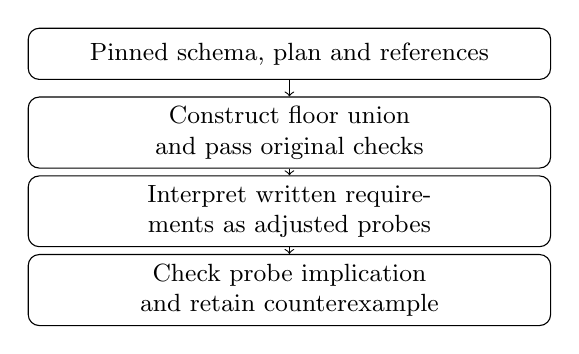
\begin{tikzpicture}[every node/.style={draw,rounded corners,align=center,font=\small,text width=6.4cm,minimum height=.65cm}]
\node (a) at (0,0) {Pinned schema, plan and references};
\node (b) at (0,-1) {Construct floor union and pass original checks};
\node (c) at (0,-2) {Interpret written requirements as adjusted probes};
\node (d) at (0,-3) {Check probe implication and retain counterexample};
\draw[->] (a)--(b); \draw[->] (b)--(c); \draw[->] (c)--(d);
\end{tikzpicture}
\caption{Native plan acceptance and requirement interpretation are separate evidence steps.}
\Description{Four steps flow downward from pinned artifacts to accepted candidate construction, requirement probes and symbolic counterexamples.}
\label{fig:workflow}
\end{figure}

\subsection{Requirement-sensitive probes}
Every probe requires an active project, auditor membership and different departments. It selects one original role and excludes the other original role, DataManager and SponsorRepresentative to avoid ambiguity about intersecting role-specific restrictions. ClinicalResearcher probes require sufficient clearance and a non-HighlyRestricted document. PrincipalInvestigator probes require low network risk and a compliant device.

The relaxed-clearance variant uses clearance at least three rather than strictly above three. Consent is required for Edit in the consent and full-expansion variants. ClinicalResearcher probes avoid Phase-3 in the study-phase and full-expansion variants. In the embargo variant they require the request time to reach the embargo boundary. The PI embargo exemption is retained. The device restriction for HighlyRestricted documents is already satisfied by the PI conditions; CR probes exclude those documents.

Each probe is schema-validated and checked for satisfiability through a non-deny-all result. A vacuous or invalid probe is not counted as covered. The auditor-removal variant supplies a negative control: its four probes are intentionally prohibited, not four missing positive requirements.

\subsection{Controls and output interpretation}
We add the adjusted probes to each floor-union candidate and rerun all original checks. This tests compatibility with the stored constraints; adding a probe does not independently validate its natural-language interpretation. In the removal control the addition should be rejected. We also reverse floor-policy order and test semantic equivalence for View and Edit.

Cedar's symbolic command can return process success for both a verified property and a counterexample. The audit therefore parses the formal verdict instead of treating a zero exit code as a proof. Timeouts and unknown outputs are retained as tool errors. We report descriptive counts only. Related variants and individual requests are not independent observations, so no confidence interval, significance test or population estimate is computed.

\section{Results}
Table~\ref{tab:results} is generated from the raw receipt. All 11 candidates validate and satisfy their original plans, totaling 149 checks. All 44 probes validate and are nonempty. The ten exception-retaining scenarios contain 40 positive probes: six are covered and 34 have an accepted-candidate counterexample. All ten contain at least one such omission. The removal scenario contributes four intentional-denial controls, excluded from that denominator.

% GENERATED_TABLE_BEGIN
\begin{table}[t]
\centering\small\setlength{\tabcolsep}{3pt}
\caption{Native clinical-family results. C: covered probes; O: omitted probes. Aug.: augmented candidate satisfies original plan. Removal is a negative control.}
\label{tab:results}
\begin{tabular}{lrrrr}
\toprule Scenario & Checks & C & O & Aug.\\\midrule
base & 13/13 & 1 & 3 & Pass \\
add\_consent & 11/11 & 0 & 4 & Pass \\
add\_datamanager & 11/11 & 1 & 3 & Pass \\
add\_export & 15/15 & 0 & 4 & Pass \\
add\_sponsor & 13/13 & 1 & 3 & Pass \\
add\_study\_phase & 15/15 & 1 & 3 & Pass \\
dual\_forbid & 14/14 & 0 & 4 & Pass \\
full\_expansion & 19/19 & 0 & 4 & Pass \\
relax\_clearance & 11/11 & 1 & 3 & Pass \\
remove\_auditor & 12/12 & -- & -- & Reject \\
temporal\_embargo & 15/15 & 1 & 3 & Pass \\
\bottomrule\end{tabular}
\end{table}
% GENERATED_TABLE_END

The base covers the CR View slice, but not CR Edit or either PI slice. The consent variant covers none of the four. DataManager, sponsor, relaxed-clearance and temporal variants each cover CR View only. The study-phase variant covers PI View only. Export, dual-forbid and full-expansion variants cover none of the four tested slices. These counts describe universal probe implication: an omitted slice has at least one counterexample, not necessarily denial of every request in that slice.

In all ten exception-retaining scenarios, the augmented policy satisfies every original check. In the auditor-removal control, augmentation violates four original ceiling checks. This result is consistent with the control's explicit removal of the exception. All 22 action-specific order-reversal equivalence checks succeed. Figure~\ref{fig:counts} displays the positive-probe counts without treating them as a prevalence estimate.

% GENERATED_FIGURE_BEGIN
\begin{figure}[t]
\centering
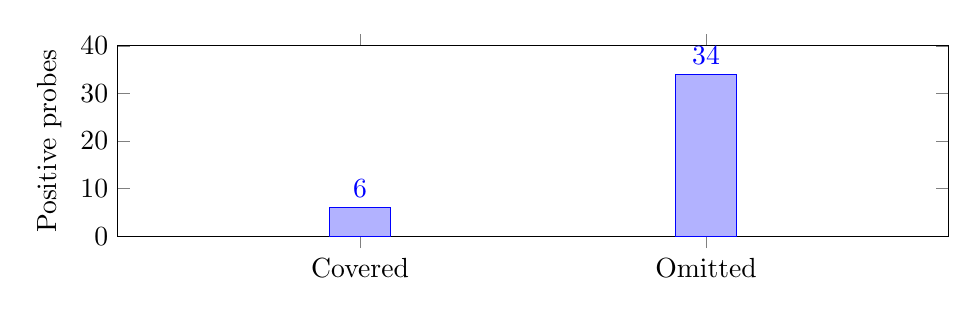
\begin{tikzpicture}
\begin{axis}[ybar,width=\columnwidth,height=4cm,ymin=0,ymax=40,
symbolic x coords={Covered,Omitted},xtick=data,ylabel={Positive probes},
nodes near coords,bar width=22pt,enlarge x limits=.7]
\addplot coordinates {(Covered,6) (Omitted,34)};
\end{axis}\end{tikzpicture}
\caption{Auditor probe coverage in ten related exception-retaining scenarios. Counts are not a benchmark-wide prevalence estimate.}
\Description{Bar chart showing six covered and thirty-four omitted positive auditor probes.}
\label{fig:counts}
\end{figure}
% GENERATED_FIGURE_END

The original concrete witness provides an additional evaluator check. A PI plus GlobalAuditor, in a different department, with low risk and a compliant device, requests View on an active project. The deficient consent candidate denies and the interpreted target allows, with schema-based request validation enabled. That request demonstrates realizability of the motivating example; it is not a replay of every symbolic witness from the family audit.

\section{Discussion}
The distinction between a necessary condition and a required permission is decisive. A ceiling permitting auditor access merely allows a candidate to grant it. It does not require the grant. Similarly, an action can be live because of same-department requests while the cross-department workflow remains unavailable. A role/action coverage table can expose this mismatch more clearly than an undifferentiated count of successful checks.

The base-to-consent comparison gives a concrete artifact relationship: a positive auditor View obligation present in the base plan is absent in the consent plan, while the prose retains the exception. We do not establish the historical process that caused this difference. Other variants add or narrow behavior, so mechanically copying all base obligations would be unsound. The failing removal control demonstrates that adding access indiscriminately is not a valid repair strategy.

The findings do not invalidate AutoCedar's statement of convergence against its formal targets. We have not inspected the actual generated policies for these cases. A model could produce the intended auditor behavior despite an incomplete acceptance plan. Conversely, a plan-level pass alone is insufficient evidence for that behavior. Future re-evaluation should report target adequacy and candidate conformance separately.

For benchmark maintenance, the useful artifact is a trace from each unchanged or narrowed requirement to an explicit positive or negative obligation, supported by a realizable witness or counterexample. This is an application of established testing ideas. Our empirical observation is the demonstrated gap in the pinned clinical family, not a claim that traceability, symbolic implication or regression checking is new.

\section{Threats to Validity}
\textbf{Interpretation.} Requirements were interpreted using AI tooling without independent human adjudication. Some prose uses necessary-condition language. We rely on the explicit auditor exception together with the stated role access paths, and restrict probes to avoid mixed-role ambiguity. Alternative intended underspecification could change the classification from defect to documentation mismatch. The native implication results remain true regardless of that interpretation.

\textbf{Selection and dependence.} The family was chosen after discovery of an omission, and several cases informed protocol design. A fixed inventory limits further cherry-picking but does not remove that selection bias. The related scenarios cannot establish general prevalence. New roles, Export probes, other requirement classes and other benchmark families are excluded.

\textbf{Implementation.} The probe generator and interpretation share assumptions. Native validation, complete-plan checks, negative controls, policy-order equivalence and an independent receipt checker reduce some implementation risks but do not prove the audit software correct. Exact Cedar 4.10.0 reproduction and a second solver are not available in this release.

\textbf{Ecological validity.} There are no real patient records, deployed systems, human participants, user outcomes or model-performance measurements. The candidate is constructed to challenge the plan, not to imitate a likely model output. Consequently, no operational harm rate or AI failure rate is claimed.

\balance
\section{Reproducibility and Research Status}
The repository provides the frozen inventory, scripts, input hashes, candidate and probe policies, native command receipts and manuscript generation checks~\cite{ours}. Derived floor-union policies retain upstream Apache-2.0 licensing and notices. Original work remains unlicensed pending an author decision. Downloaded papers, credentials and tool binaries are excluded from the distributable archive.

AI tools assisted literature retrieval, implementation and manuscript drafting. This does not constitute independent expert review. This manuscript is a technical case-study preprint candidate, not an accepted journal article. Its method is established; the possible contribution is the pinned empirical evidence. External-family replication and independent interpretation review would strengthen a journal submission.

\section{Conclusion}
In one pinned CedarBench clinical family, all 149 original checks accept the constructed candidates, yet 34 of 40 interpreted auditor-access probes have counterexamples. Adjusted positive obligations remain compatible with the ten exception-retaining plans, while intentional exception removal correctly rejects their addition. The result illustrates why acceptance-plan success should be reported separately from coverage of written requirements. It provides a reproducible case study, with explicit limits on novelty, generalization and model-performance claims.

\begin{thebibliography}{9}
\bibitem{autocedar} Adarsh Vatsa, Sachi Shome, Yingming Zhou, and William Eiers. 2026. AutoCedar: An Agentic Framework for Verifier-Guided Access Control Policy Synthesis. arXiv:2607.03656v1. \url{https://arxiv.org/abs/2607.03656}
\bibitem{cedar} Joseph W. Cutler et al. 2024. Cedar: A New Language for Expressive, Fast, Safe, and Analyzable Authorization (Extended Version). arXiv:2403.04651v2. \url{https://arxiv.org/abs/2403.04651}
\bibitem{nist} Vincent C. Hu, Rick Kuhn, and Dylan Yaga. 2017. Verification and Test Methods for Access Control Policies/Models. NIST SP 800-192. \url{https://doi.org/10.6028/NIST.SP.800-192}
\bibitem{martin} Evan Martin and Tao Xie. 2006. Toward Systematic Testing of Access Control Policies. \url{https://prolangs.cs.vt.edu/rutgers/meetings/masplas06/papers/5_Martin.pdf}
\bibitem{hwang} JeeHyun Hwang, Tao Xie, Donia El Kateb, Tejeddine Mouelhi, and Yves Le Traon. 2012. Selection of Regression System Tests for Security Policy Evolution. In ASE, 266--269. \url{https://doi.org/10.1145/2351676.2351719}
\bibitem{artifact} AutoCedar Authors. 2026. Cedar synthesis engine and CedarBench artifacts. Commit \texttt{0201565abf5993e258764d3f0ef83a59d3b4962e}. \url{https://github.com/neselab/cedar-synthesis-engine}
\bibitem{ours} Ezekiel Ologunde. 2026. Auditor obligation audit: source, protocol and receipts. \url{https://github.com/ezekielologunde/remediation-evidence-interfaces}
\end{thebibliography}
\end{document}
